\renewcommand{\inputfile}{\version\ - edited 2008-06-26 appeKSeDetails}

Truncating the infinite tower of equations \refeq{expan} by setting $a_k=0$ for $k>N$
allows one to numerically integrate it. There are three technical issues that need some attention
in order to accurately and efficiently simulate Kuramoto-Sivashinsky: evaluation of
the nonlinear part, number of modes retained and stiffness.

\subsection{Pseudospectral method}
\label{sec:ksPseudo}

The linear part of \KSe\ is conveniently diagonal in the Fourier basis, see \refeq{expan}.
The nonlinear part can be evaluated directly from the finite order truncation of \refeq{expan},
see \refsect{sec:ksReal} for an implementation. By using a pseudo-spectral method though, one
can take advantage of the efficiency of the Fast Fourier Transform in evaluating the
nonlinear part. For \KSe\ this is done by  applying a discrete Fourier transform to \refeq{ks} and
taking into account that the Fourier operator is linear so that we can rewrite \refeq{expan}
in the following way
\beq
\dot{a}_k= ( q_k^2 - q_k^4 )\, a_k
    - i \frac{q_k}{2} \mathcal{F}\left[\left(\mathcal{F}^{-1}\left[a\right]\right)^2\right]_k \,,
	\label{eq:ksPseudo}
\eeq
where $\mathcal F$ is the discrete Fourier transform,
\beq
  a_k = \mathcal{F}[u]_k = \sum_{n = 0}^{N-1} u(x_n)
  e^{-i q_k x_n}\,,\qquad u(x_n) = \mathcal{F}^{-1}[a]_n
  = \frac{1}{N}\sum_{k = 0}^{N-1} a_k e^{i q_k x_n}\,,
\eeq
with $x_n = 2\pi\tildeL n/N$ and $a_{N-k} = a^\ast_k$ from the reality condition \refeq{eq:astar}
and thus calculation of the discrete Fourier transform involves $N-1$ real variables.

Since we have set $a_0=0$ to eliminate Galilean invariance and the modes with $k<0$
are redundant from \refeq{eq:astar}, we can evaluate then nonlinear part in \refeq{expan}
in $N/2-1$ complex variables. The operation would correspond to multiplication of a real $(N-2)\times(N-2)$
matrix by a $N-2$-dimensional vector, while calculating just the forward Fourier transform
would require the multiplication of a $(N-1)\times(N-1)$ matrix by a $N-1$-dimensional vector.
In any case the operation count is $\Order{N^2}$, but with the pseudo-spectral method we need two
of them. The power of the pseudo-spectral method lies in the existence of the Fast Fourier Transform (FFT)
algorithm that performs the discrete Fourier transform in $\Order{N log_2 N}$ operations therefore
providing substantial performance advantage to the pseudo-spectral method. The FFT algorithm
has been rediscovered many times, apparently starting with Gauss, see \refref{Press96} for references
and a presentation of the algorithm. In our implementation we have used the FFTW package \refref{Frigo05}.

\subsection{Stiffness}

The second issue one has to deal with in integrating \refeq{expan} is due to the linear part.
The term $k^4$ that appears in the linear part means that the timescales on which the first
and the $N$'th mode evolve is very different even for $N$ of the order of $10$. This
is termed stiffness, see \refref{Press96} for a nice discussion. In practice, unless taken care
of by the integration method, it forces us to follow the evolution of the equation in the
fastest time-scale in order to maintain stability of the integration routine, thus imposing an
impractically small stepsize. There are different approaches to dealing with stiffness,
see \refref{ks05com} for a comparison of algorithms that can be used to integrate stiff PDEs.

The algorithm that we have found very efficient and accurate in our numerical explorations
is Exponential Time Differencing with fourth order Runge-Kutta timesteping (ETDRK4)
introduced in \refref{cox02jcomp} and further developed in \refref{ks05com}, which we have
followed in our implementation. The essence of the method is that it treats the linear
and nonlinear part separately, applying an integrating factor to the linear part to eliminate
the effect of stiffness.

As the method requires the computation of prefactors that depend on the linear part of
the equation, we found it inconvenient to implement an adaptive stepsize control. Instead,
we check the results of integration against decreasing the timestep, especially the
robustness of relative periodic and periodic orbits found in \refchap{chap:kseStSp}.

\subsection{Truncation}

Another decision one has to make is how many modes to retain
in \refeq{eq:ksPseudo}. One has to keep in mind that we want
accurate solutions to the original PDE, we do not just
consider a truncation to finite $N$ on its own right. Due to
the hyperviscous damping $u_{xxxx}$, long time solutions of
KS equation are smooth, $a_k$ drop off fast with $k$, and
truncations of \refeq{expan} to $16 \leq N \leq 128$ terms
yield accurate solutions for system sizes considered here.
Robustness of the long-time dynamics of KS as a function of
the number of Fourier modes kept in truncations of
\refeq{expan} is, however, a subtle issue.  Adding an extra
mode to a truncation of the system introduces a small
perturbation in the space of dynamical systems.  However, due
to the lack of structural stability both as a function of
truncations $N$, and the system size \tildeL, a small
variation in a system parameter can (and often will) throw
the dynamics into a different asymptotic state.  For example,
asymptotic attractor which appears to be chaotic in a
$N$-dimensional \statesp\ truncation can collapse into an
attractive cycle for $(N\!+\!1)$-dimensions. Therefore we
always evaluate the robustness of our results by increasing
the number of modes. For instance, when we compute an
unstable \po\ we check that its period and stability
eigenvalues remain within the desired accuracy when
recomputed in a higher-dimensional truncation.

For system size $L=22$ all results presented here were computed using
a $128$-point spatial discretization, corresponding to $N=64$ complex Fourier modes
(with $a_0=0$ though). Note that going back and forth in Fourier and physical
space in \refeq{eq:ksPseudo} one has to worry about the effect of aliasing
on the results of the integration. Since our computations are relatively cheap
we circumvent this difficulty by keeping enough modes so that at least half
of the modes remain close to zero during a calculation. We also confirm our
results against direct evaluation of the truncation of \refeq{expan}, see \refsect{sec:ksReal}.


% \section{\KSe\ according to Evangelos}
% $Author$ $Date$

% The \KSe\ % (KSe)
% reads:
%  \beq
%   u_t=(u^2)_x-u_{xx}- u_{xxxx} \, ,
%   \label{eq:KS0}
%  \eeq
%
%  We assume periodic boundary conditions on the $x\in [0,2\pi \tilde{L}]$
%  interval:
%  \beq
%    u(x+2\pi\tilde{L},t)=u(x,t) \, ,
%  \eeq
%  which allows a Fourier series expansion:
%  \beq
%   u(x,t)=\sum_{k=-\infty}^{+\infty} a_k (t) e^{ i k x / \tilde{L}} \, .
%   \label{eq:Fourier}
%  \eeq

\section{Calculating stability of equilibria}
\label{sec:ksReal}


To calculate stability of equilibrium, the matrix
\beq
  A(a_q) = \left.\frac{\partial v}{\partial a}\right|_{a=a_q}
\label{eq:StabMat}
\eeq
has to be evaluated, either numerically or analytically. In \KS\
we can obtain $A(a_q)$ efficiently for numerical
purposes by using the linearity of the
Fourier transform, as we did to get \refeq{eq:ksPseudo},
see \refref{SCD07}.

In what follows we derive an analytical expression for it,
as one might find it useful for the study of bifurcation problems,
or, in our case, to cross-check the results of the pseudo-spectral method.
%  Since $u(x,t)$ is real,
%  \beq
%   a_{k}=a^*_{-k} \, .
%   \label{eq:a*}
%  \eeq
%  Substituting \refeq{eq:Fourier} into \refeq{eq:KS} we get:
%  \beq
%   \dot{a}_k=(q_k)^2\left(1-(1/\tildeL)^2 k^2\right)a_k
%         + i (q_k)  \sum_{m=-\infty}^{+\infty}a_m a_{k-m} \, .
%   \label{eq:Fcoef}
%  \eeq
%
%  From \refeq{eq:Fcoef} we note that $\dot{a}_0=0$ and thus $a_0$ is an integral
%  of the equations or, from \refeq{eq:Fourier}, the average of the solution $\int dx u(x,t)$
%  is a constant. Due to galilean invariance we may set $a_0=0$ without loss of generality
%  and we only have to compute $a_k$'s with $k\geq 1$. % Explain this in detail somewhere.
 To do so, we have to split \KS\ equation into real and imaginary
 parts\ES{or consider $a$ and $a^{*}$ as independent variables.}.
 Truncating the infinite tower of equations \refeq{expan} by setting $a_k=0$ for $k>N$,
 using the identity \refeq{eq:astar} and splitting the
 resulting equations into real and imaginary part by setting $a_k=b_k+i c_k$, we have
 \bea
  \dot{b}_k & = & q_k^2\left(1- q_k^2 \right)b_k  \continue
    & & + \frac{q_k}{2} \left(\sum_{m=1}^{k-1}c_m b_{k-m}+\sum_{m=k+1}^{N}c_m b_{m-k}
                    -\sum_{m=1}^{N-k}c_m b_{k+m} \right)  \continue
    & & + \frac{q_k}{2} \left(\sum_{m=1}^{k-1}b_m c_{k-m}-\sum_{m=k+1}^{N}b_m c_{m-k}
                    +\sum_{m=1}^{N-k}b_m c_{k+m} \right)
  \label{eq:tmp:b-Trunc}
 \eea
 \bea
   \dot{c}_k & = & q_k^2\left(1- q_k^2 \right)c_k  \continue
    & & + \frac{q_k}{2}\left( \sum_{m=1}^{k-1}c_m c_{k-m}-\sum_{m=k+1}^{N}c_m c_{m-k}
                    -\sum_{m=1}^{N-k}c_m c_{k+m} \right)    \continue
    & & - \frac{q_k}{2} \left(\sum_{m=1}^{k-1}b_m b_{k-m}+\sum_{m=k+1}^{N}b_m b_{m-k}
                    +\sum_{m=1}^{N-k}b_m b_{k+m} \right)
   \label{eq:tmp:c-Trunc}
 \eea
 where now only terms $c_{k},b_{k}$ with $0<k<N$\ES{Changed $d$ to $N$.} appear. Observe that
 \beq
    \sum_{m=1}^{N-k}c_m b_{k+m} = \sum_{m=k+1}^{N}b_m c_{m-k}\,,
 \eeq
 \etc\ and thus \refeq{eq:tmp:b-Trunc} and \refeq{eq:tmp:c-Trunc} simplify to
  \bea
  \dot{b}_k & = & q_k^2\left(1- q_k^2 \right)b_k  \continue
    & & + \frac{q_k}{2} \left(\sum_{m=1}^{k-1}c_m b_{k-m}-2\sum_{m=1}^{N-k}c_m b_{k+m} \right)  \continue
    & & + \frac{q_k}{2} \left(\sum_{m=1}^{k-1}b_m c_{k-m}+2\sum_{m=1}^{N-k}b_m c_{k+m} \right)
  \label{eq:b-Trunc}
 \eea
 \bea
   \dot{c}_k & = & q_k^2\left(1- q_k^2 \right)c_k  \continue
    & & + \frac{q_k}{2}\left( \sum_{m=1}^{k-1}c_m c_{k-m}-2\sum_{m=1}^{N-k}c_m c_{k+m} \right)  \continue
    & & - \frac{q_k}{2}\left( \sum_{m=1}^{k-1}b_m b_{k-m}+2\sum_{m=1}^{N-k}b_m b_{k+m} \right)\,.
   \label{eq:c-Trunc}
 \eea
 As discussed in \refsect{sec:ksPseudo} such expressions are not as efficient as using a pseudo-spectral
implementation, but we use them for comparison purposes, to detect possible issues in our pseudo-spectral
integrator due to  aliasing or the FFT implementation\ES{For instance I was able to find using this that the FFT in numerical recipes basically sucks.}.

 To calculate the matrix $A_{ij}(a) \equiv \frac{\partial v_i(x)}{\partial x_j}$  we need to consider the four matrices $\frac{\partial \dot{b}_k}{\partial b_j},\frac{\partial \dot{b}_k}{\partial c_j},\frac{\partial \dot{c}_k}{\partial b_j},\frac{\partial \dot{c}_k}{\partial c_j}$. We begin with
 \bea
    \frac{\partial \dot{c}_k}{\partial c_{j}}  =
        q_k^2\left(1- q_k^2 \right) \delta_{kj}
            - \frac{q_k}{2}\frac{\partial}{\partial c_j}\left( \sum_{m=1}^{k-1}c_m c_{k-m}-2\sum_{m=1}^{N-k}c_m c_{k+m} \right) \,.
 \eea
 Consider the second term:
 \bea
    - \frac{q_k}{2}\frac{\partial}{\partial c_j}\left( \sum_{m=1}^{k-1}c_m c_{k-m}-2\sum_{m=1}^{N-k}c_m c_{k+m} \right) & = &
        - \frac{q_k}{2} \sum_{m=1}^{k-1} \left(\delta_{m,j} c_{k-m}+c_m \delta_{k-m,j} \right) \continue
                        & & +  q_k\sum_{m=1}^{N-k} \left(\delta_{m,j} c_{k+m}+c_m \delta_{k+m,j}\right)
 \eea
 We need to consider two cases separately:
 \begin{itemize}
    \item $k\leq j$
        \bea
             -\frac{q_k}{2}\frac{\partial}{\partial c_j}\left( \sum_{m=1}^{k-1}c_m c_{k-m}-2\sum_{m=1}^{N-k}c_m c_{k+m} \right) & = &
                    -\frac{q_k}{2}( 0+0 ) + q_k (c_{k+j} + c_{j-k}) \continue
                & = &    q_k (c_{k+j}-c_{k-j})
        \eea
    \item $k > j$
        \bea
             -\frac{q_k}{2}\frac{\partial}{\partial c_j}\left( \sum_{m=1}^{k-1}c_m c_{k-m}-2\sum_{m=1}^{N-k}c_m c_{k+m} \right) & = &
                    -\frac{q_k}{2}(c_{k-j} + c_{k-j} ) + q_k (c_{k+j}  + 0 ) \continue
                & = &   q_k (c_{k+j}-c_{k-j})
        \eea
 \end{itemize}
 and thus
 \beq
    \frac{\partial \dot{c}_k}{\partial c_{j}} =  q_k^2\left(1- q_k^2 \right)\delta_{kj} +  q_k (c_{k+j}-c_{k-j})
 \eeq

 Following the above procedure
 \beq
    \frac{\partial \dot{c}_k}{\partial b_{j}} =   q_k ( b_{k+j}+b_{k-j} )\,,
 \eeq
 \beq
    \frac{\partial \dot{b}_k}{\partial b_{j}} =  q_k^2\left(1- q_k^2 \right)\delta_{kj} -  q_k (c_{k+j} + c_{k-j}) \,,
 \eeq
 \beq
    \frac{\partial \dot{b}_k}{\partial c_{j}} =  q_k (b_{k+j}-b_{k-j}) \,.
 \eeq


% In terms of the system size $ 2\pi L$, the only length scale available,
% the dimensions of terms in \refeq{ks} are
% $ %\[
% [x]=L
% $, $%\,,\quad
% [t]=L^2
% $, $%\,,\quad
% [u]=L^{-1}
% $, $%\,,\quad
% [\nu]=L^2
% \,.
% $ %\]
% What is the non-dimensional ``Rayleigh'' number for the
% \KS\ system?
%  Scaling out the ``viscosity'' $\nu$
% \[
% x \to x \nu^{\frac{1}{2}}
% \,,\quad
% t \to t \nu
% \,,\quad
% u \to u \nu^{-\frac{1}{2}}
% \,,
% \]
% brings the \KSe\ \refeq{ks}
% to a non-dimensional form
% \beq
% u_t=(u^2)_x-u_{xx}- u_{xxxx}
% \,,\qquad
%   x \in  [0,L\nu^{-\frac{1}{2}}] = [0,2\pi\tilde{L}]
% \,.
% \ee{ks-L}
% In this way the ``viscosity'' $\nu$
% and the system size $L$ are trade in for a single
% dimensionless system size parameter
% \beq
%   \tilde{L}={L}/{(2 \pi \sqrt{\nu})}
% % \tilde{L}=\frac{L}{2 \pi \sqrt{\nu}}
% % \,,
% \ee{tildeL}
% which plays the role of a ``Reynolds number''
% for the \KS\ system.

% In the literature sometimes
% $L$ is used as the system parameter, with $\nu$ fixed to $1$, and
% at other times $\nu$ is varied with $L$ fixed to either $1$ or $2\pi$.
% To minimize confusion,
% in what follows we shall state results of all
% calculations in units of dimensionless system size $\tilde{L}$.
% \PC{motivate $2\pi$ factor by the mean wavelength,
%     refer to the equation number}
% Note that the time units also have to be
% rescaled; if $T^*_p$ is a period
% of a periodic solution of \refeq{ks} with a given
% $\nu$ and $L=2\pi$, then
% the corresponding solution of the non-dimensionalized \refeq{ks-L}
% has period
% \beq
%  T_p= T^*_p/\nu
% \ee{Trescl}
%


% %%%%%%%%%%%%%%%%%%%%%%%%%%%%%%%%%%%%%%%%%%%%%%%%%%%%%%%%%%%%%%%%
% \begin{figure}[t] \label{f:neighborhood2w}
% \begin{center}
% (a) 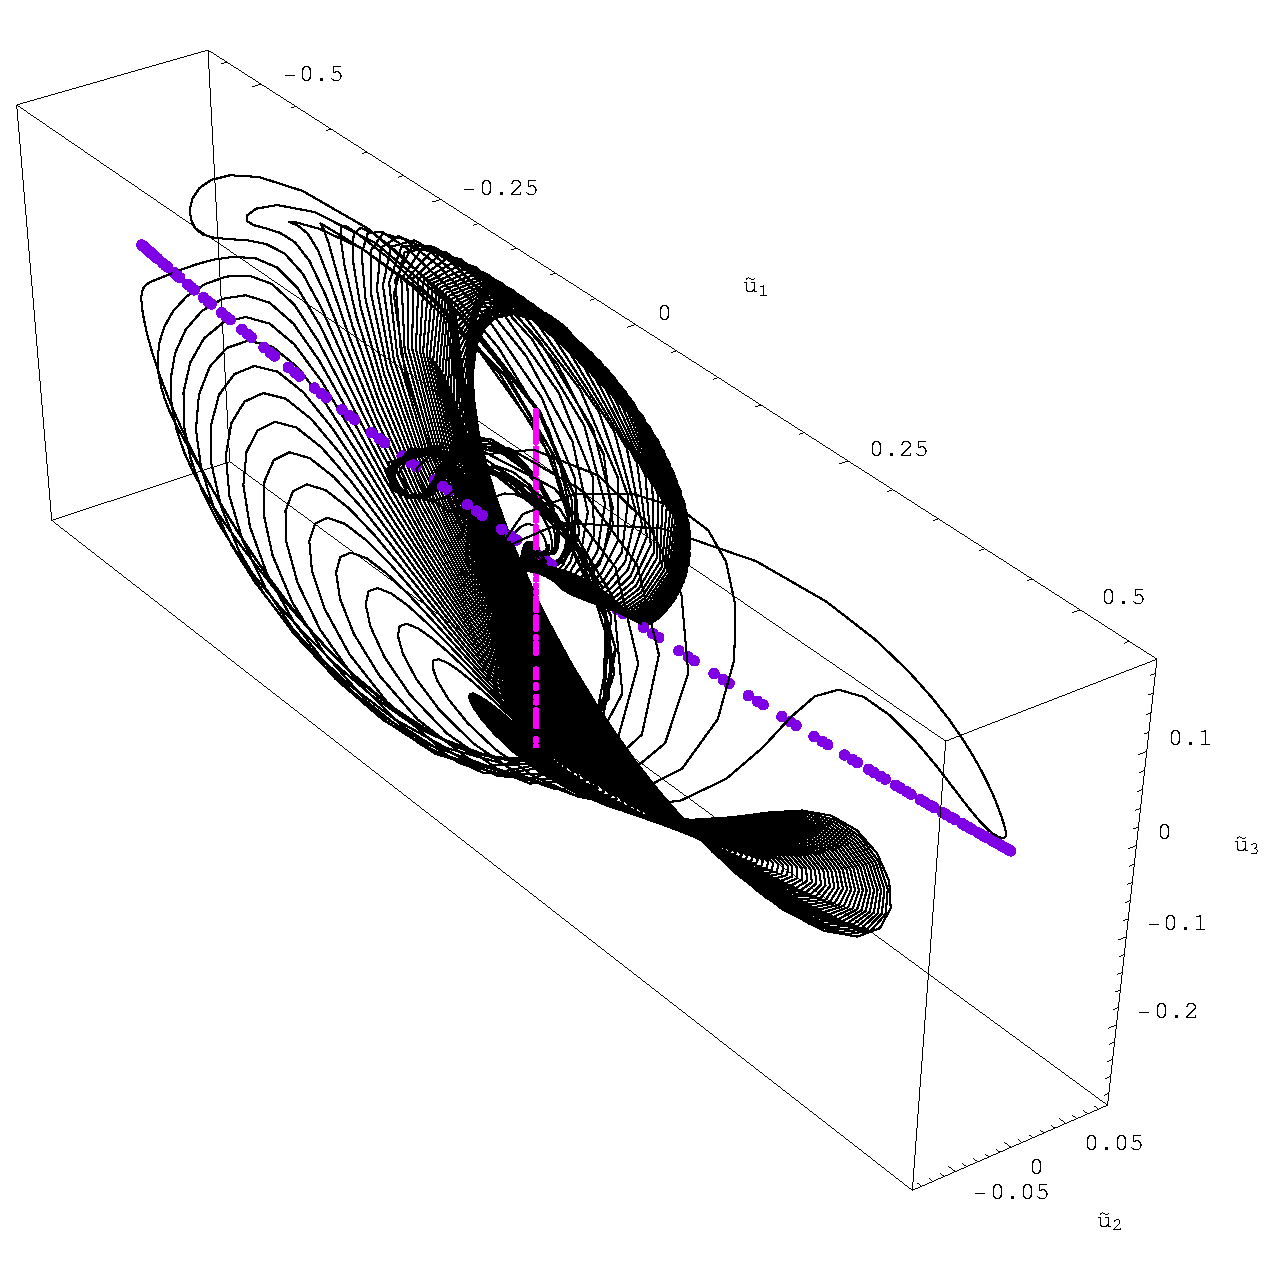
\includegraphics[width=5.0cm]{../figs/L22-2w-UnsMan}
% \hspace{0.1in}
% (b) 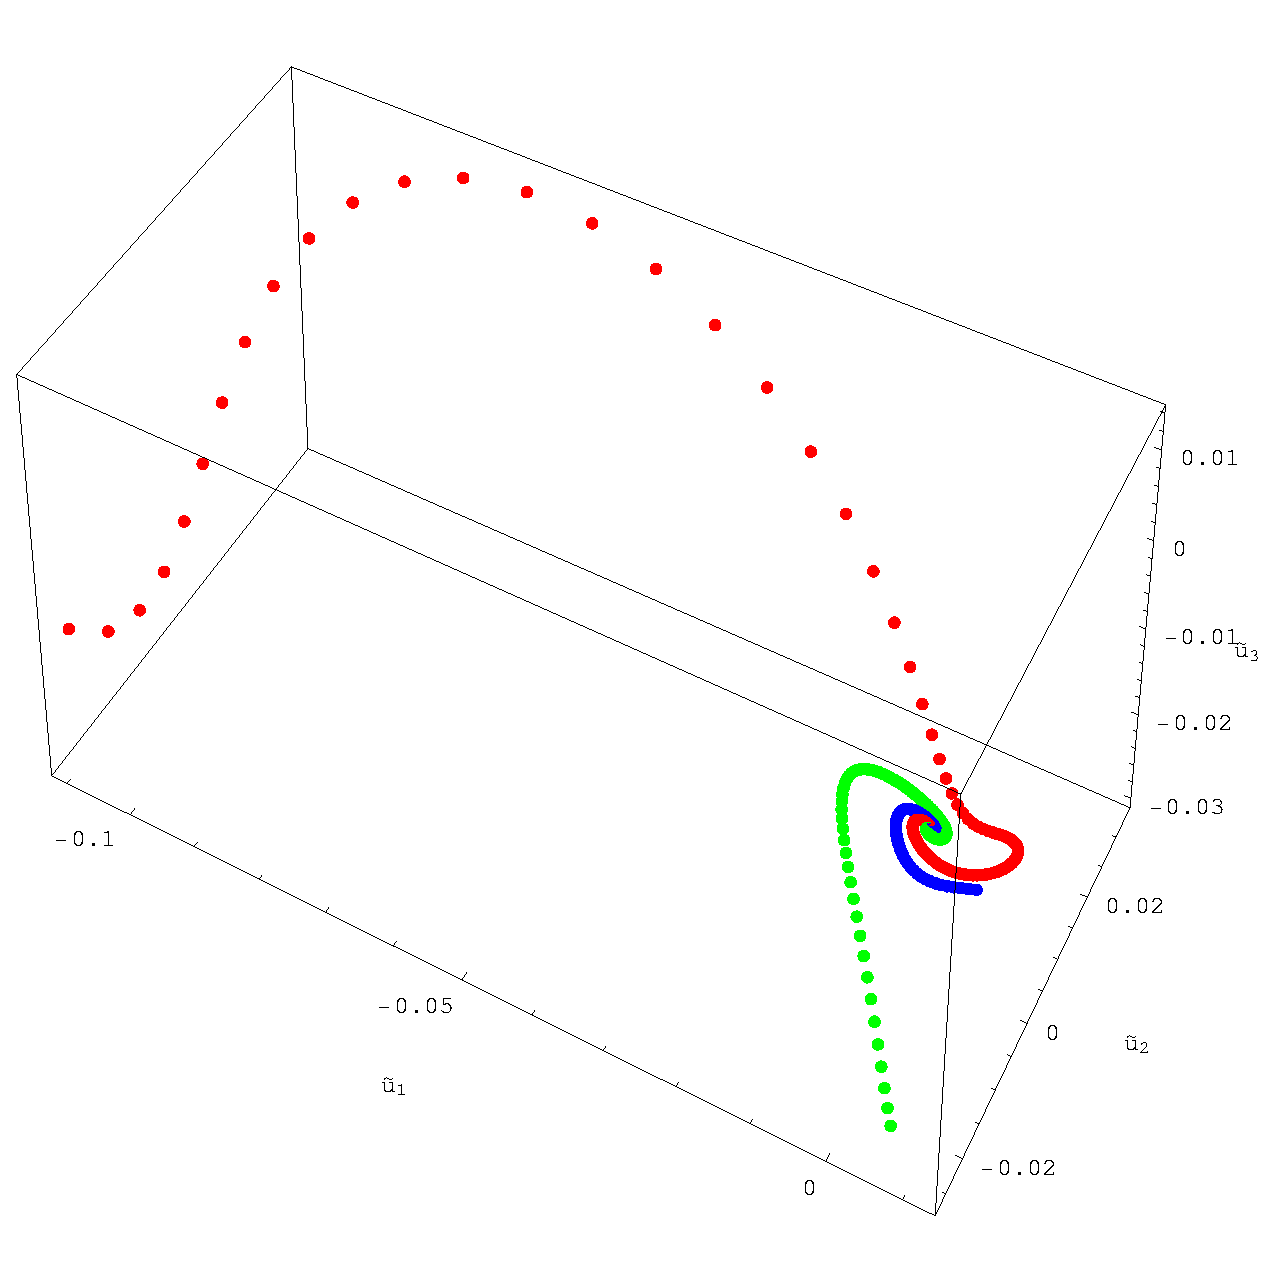
\includegraphics[width=5.0cm]{../figs/L22-2w-UnsMan-BlowUp}
% % (b) 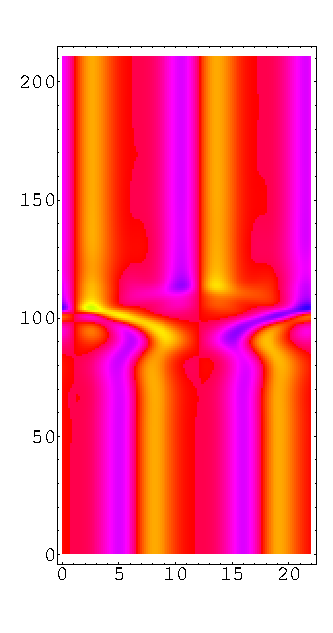
\includegraphics[width=4.0cm]{figs/L22-2w-R}
% \\
% (c) 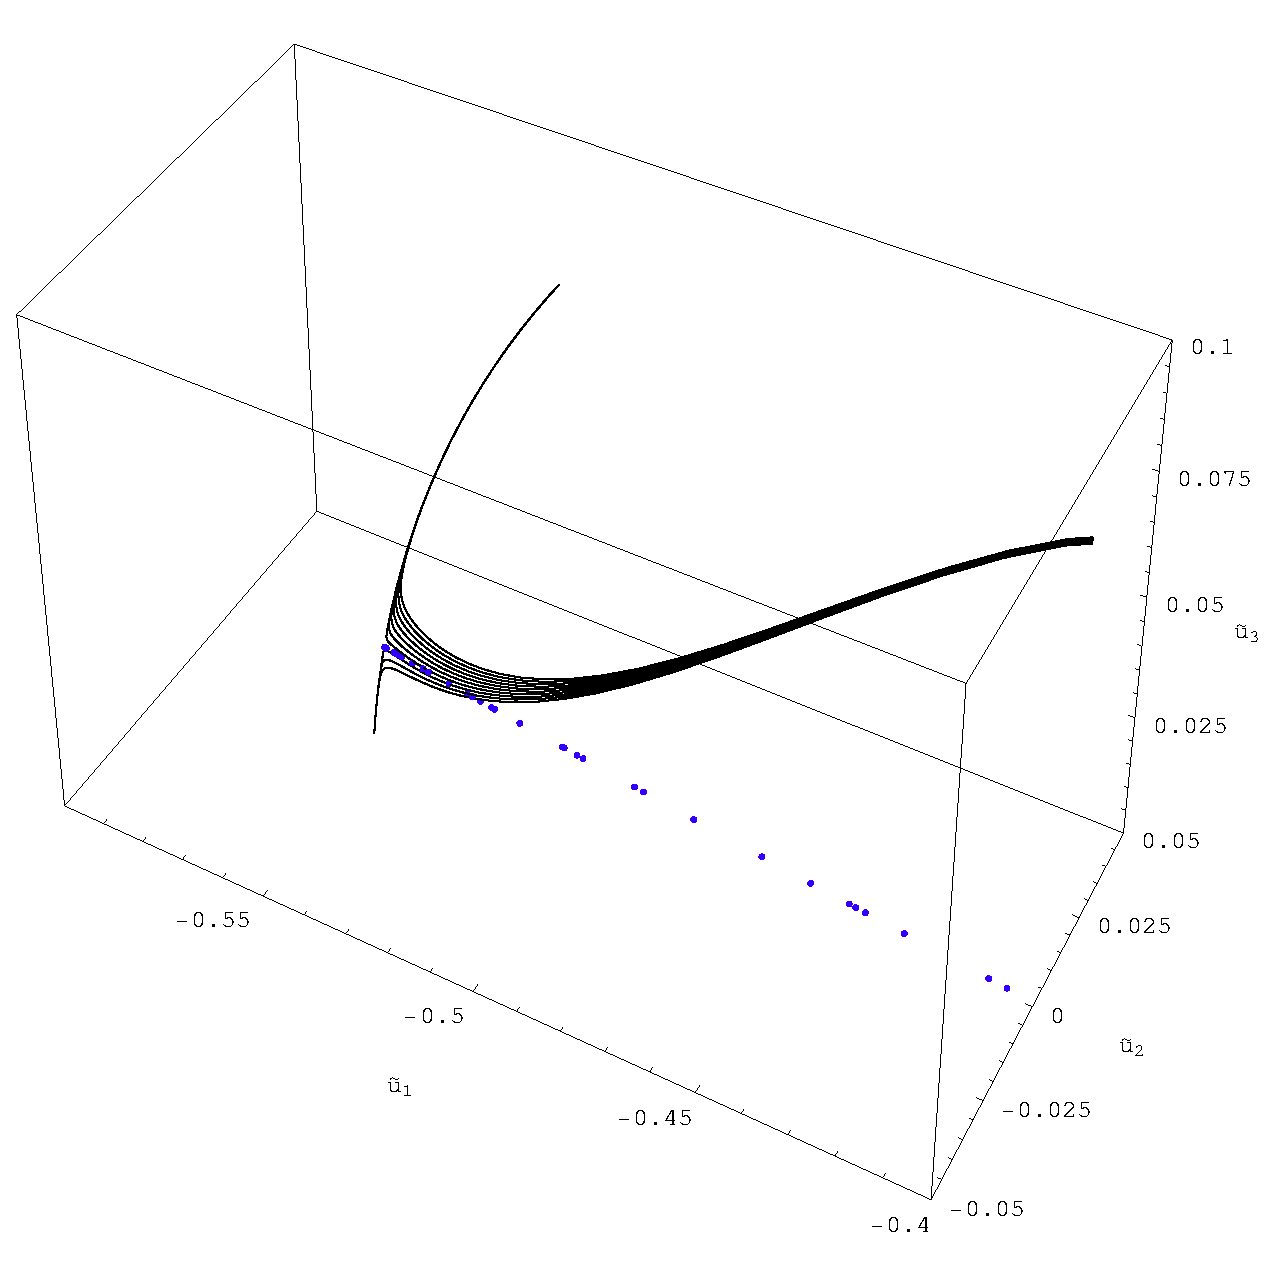
\includegraphics[width=5.0cm]{../figs/L22-2w-3w-UnsMan}
% % (c) 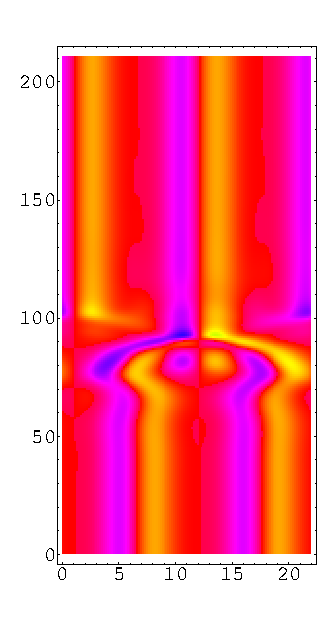
\includegraphics[width=4.0cm]{figs/L22-2w-G}
% \hspace{0.1in}
% (d)  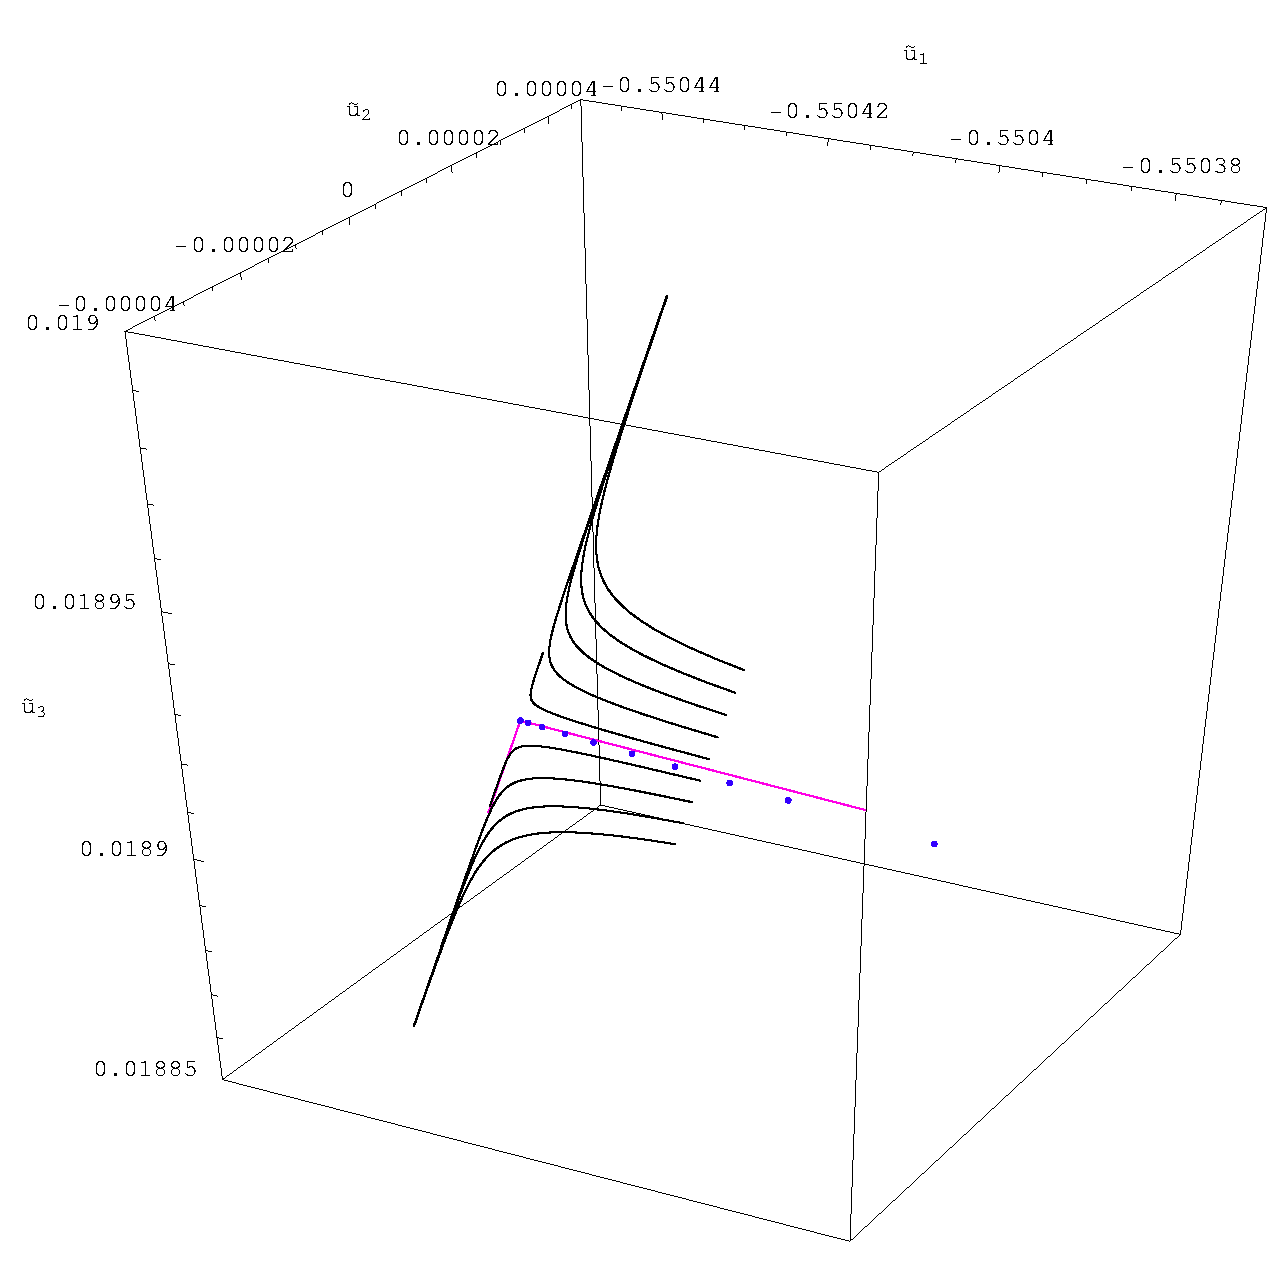
\includegraphics[width=5.0cm]{../figs/L22-2w-3w-detail}
% % (d) 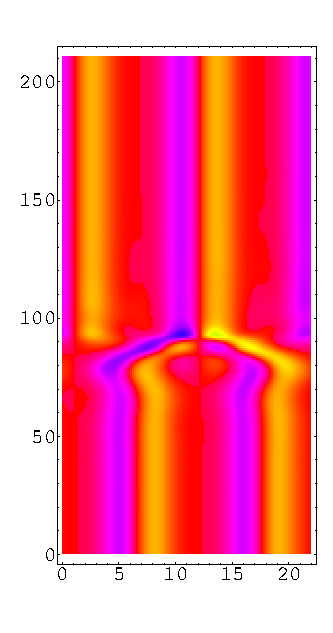
\includegraphics[width=4.0cm]{figs/L22-2w-B}
% \end{center}
% \caption{
%  Trajectories with initial conditions on the unstable subspace of
%  the \EQV{2}~\eqv.
%  (a) The coordinates $\tilde{u}_1$ and $\tilde{u}_2$
%  are along the directions defining the unstable subspace
%  and $\tilde{u}_3$  is along the real part of the eigenvector
%  corresponding to the eigenvalue $-0.271122+ i\, 0.356307$.
% The purple points represent the continuous family
%  of
% \EQV{2}~\eqva.
% % Green curve belongs to \reffig{f:rpo55}(b) % rpo22-55-4-cm.eps
% % rather than to  \reffig{f:rpo55}(a), % rpoEq22-55-4.eps?
% (b) blowup of ``homoclinic'' descent of the unstable manifold
% back into \EQV{2}~\eqv, shifted by
% $L/4$.
% (c) blowup of ``heteroclinic'' connection from
% \EQV{2} \eqv\ to \EQV{3} \eqv, with shift
% $L(1/3-1/4) = L/12$
% \PCedit{(? check)}
% to the neighborhood of the point near which the
% unstable manifold of the
% \EQV{2} \eqv\ splits. The blue points
% represent the
% \EQV{3} {\eqv} family.
% The descent is along the eigenvector of $\Lyap_4= 0.413$,
% \ESedit{(checked)}
% and splitting
% occurs along one of the
% $\Lyap_1=\Lyap_2=0.0933$
% unstable directions of the \EQV{2}~{\eqv}.
% \ESedit{(checked)}
% (d) same as (c), closer to the \EQV{3}~{\eqv}.
% The eigendirections corresponding to $\Lyap_1$
% and $\Lyap_4$ are shown in purple.
% }
% \end{figure}
% %%%%%%%%%%%%%%%%%%%%%%%%%%%%%%%%%%%%%%%%%%%%%%%%%%%%%%%%%%%%%%%%%%
